
\section*{Problema P7.12}

\renewcommand*\thesection{7.12}
\numberwithin{equation}{section}

\begin{center}
    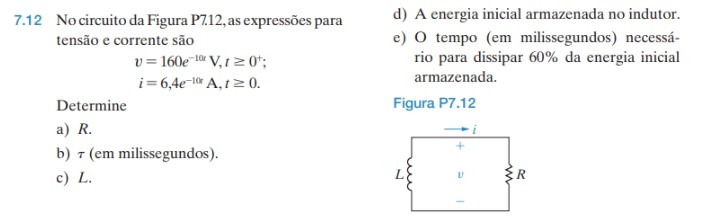
\includegraphics[scale=1.0]{P7.12.jpg}
\end{center}

\subsection*{(a)}

Aplicando análise de malhas, temos   

\[- v(t) + Ri = 0 \]

Isolando $R$,

\[ R = \frac{v(t)}{i(t)} \]

Substituindo os valores do enunciado,   

\[ R = \frac{160e^{-10t}}{6.4e^{-10t}} \]

\[ \boxed{R = 25 \;\Omega}  \]

\subsection*{(b)}

Em regime transitório CC, a função da corrente no indutor é  

\[ i(t) = i(0)e^{-\frac{t}{\tau}} \]

Onde $\tau$ é a constante de tempo. Comparando com o valor do enunciado,

\[ \boxed{\tau = \frac{1}{10} = 100 \un{ms}}   \]

\subsection*{(c)}

Usando

\[ \tau = \frac{L}{R} \logo L = R\tau \]

Temos  

\[ \boxed{L = 25\;\Omega \cdot 100\un{ms} = 2.5 \un{H}}   \]

\subsection*{(d)}

A energia em um indutor é 

\begin{equation}\label{eq:7.12.1}
    E(t) = \frac{1}{2}L[i(t)]^2
\end{equation}

Em $t =0$, temos   

\[ \boxed{E(0) = \frac{1}{2} \cdot 2.5 \cdot (6.4)^2 = 51.2 \un{J}}   \]

\subsection*{(e)}

Usando \eqref{eq:7.12.1}, vamos isolar $t$.

\[ \frac{2E(t)}{L} = [i(t)]^2 \]

\[ \sqrt{\frac{2E(t)}{L}} = i_0e^{-\frac{t}{\tau}} \]

\[ \frac{1}{i_0} \sqrt{\frac{2E(t)}{L}} = e^{-\frac{t}{\tau}} \]

\[ -\frac{t}{\tau} = \ln\left(\frac{1}{i_0} \sqrt{\frac{2E(t)}{L}}\right) \]

\[ t = - \tau \ln\left(\frac{1}{i_0} \sqrt{\frac{2E(t)}{L}}\right) \]

Para que seja dissipado $60\%$ da energia inicial do indutor, buscamos um instante $t$ para o qual a energia $E(t)$ é
$40\%$ da inicial, ou seja, 

\[ E(t) = \frac{4}{10}E(0) = \frac{4}{10}\frac{1}{2}Li_0^2  \]

Substituindo na expressão de $t$,

\[ t = - \tau \ln\left(\frac{1}{i_0} \sqrt{\frac{2\frac{4}{10}\frac{1}{2}Li_0^2}{L}}\right) \]

\[ t = - \tau \ln\left(\sqrt{\frac{2}{5}}\right) \]

\[ \boxed{t = 41.81 \un{ms}}   \]








